% 5-stage RV32I pipeline with the DBPU (matches rtl/rv32_pipeline_core.v)
% Build: cd docs/diagrams && tectonic rv32_pipeline.tex
\documentclass[tikz,border=8pt]{standalone}
\usetikzlibrary{arrows.meta,positioning,calc,fit,backgrounds}
\begin{document}
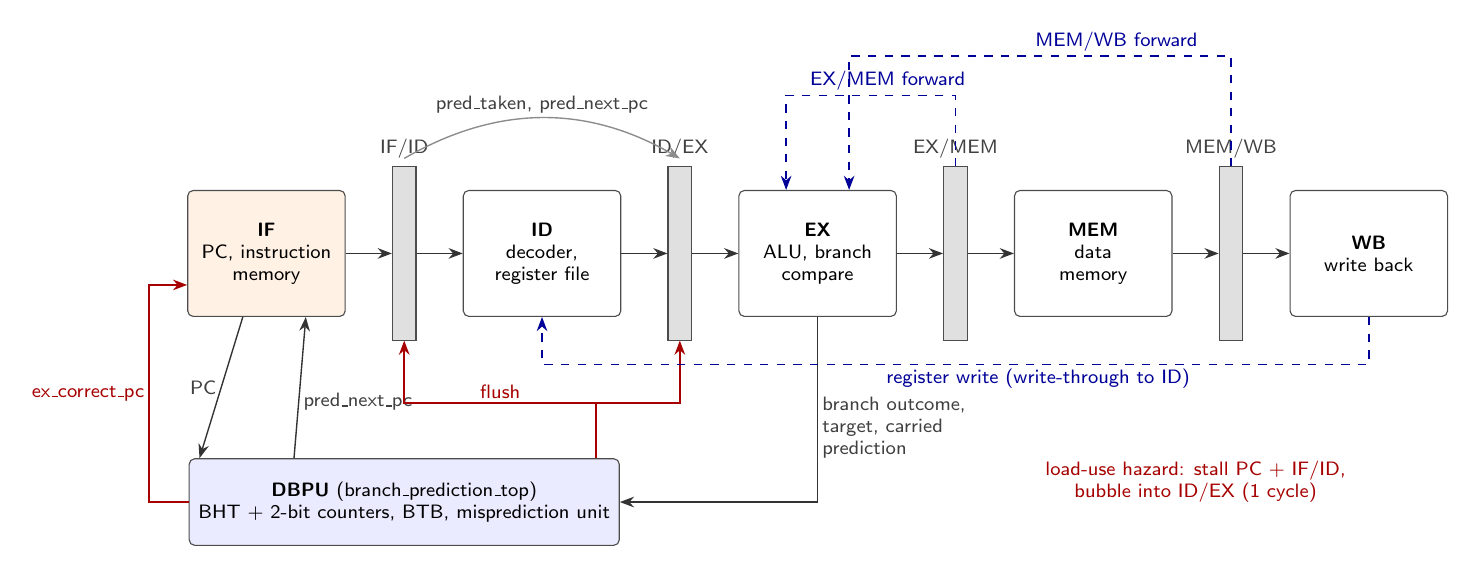
\begin{tikzpicture}[
  font=\sffamily\scriptsize, >={Stealth[length=1.8mm]},
  stage/.style={draw=black!70, rounded corners=2pt, fill=#1, minimum width=20mm, minimum height=16mm, align=center},
  stage/.default=white,
  preg/.style={draw=black!70, fill=black!12, minimum width=3mm, minimum height=22mm, inner sep=0pt},
  sig/.style={->, draw=black!80, line width=0.5pt},
  ctl/.style={->, draw=red!65!black, line width=0.6pt},
  fwd/.style={->, draw=blue!60!black, line width=0.5pt, dashed},
  lbl/.style={font=\sffamily\scriptsize, text=black!75, inner sep=1.5pt}
]
% stages
\node[stage=orange!10] (if)  at (0,0)    {\textbf{IF}\\PC, instruction\\memory};
\node[preg] (r1) at (1.75,0) {};
\node[stage]           (id)  at (3.5,0)  {\textbf{ID}\\decoder,\\register file};
\node[preg] (r2) at (5.25,0) {};
\node[stage]           (ex)  at (7.0,0)  {\textbf{EX}\\ALU, branch\\compare};
\node[preg] (r3) at (8.75,0) {};
\node[stage]           (mem) at (10.5,0) {\textbf{MEM}\\data\\memory};
\node[preg] (r4) at (12.25,0) {};
\node[stage]           (wb)  at (14.0,0) {\textbf{WB}\\write back};
\foreach \n/\t in {r1/{IF/ID}, r2/{ID/EX}, r3/{EX/MEM}, r4/{MEM/WB}}
  \node[lbl, above=1pt of \n] {\t};

\draw[sig] (if) -- (r1); \draw[sig] (r1) -- (id); \draw[sig] (id) -- (r2); \draw[sig] (r2) -- (ex);
\draw[sig] (ex) -- (r3); \draw[sig] (r3) -- (mem); \draw[sig] (mem) -- (r4); \draw[sig] (r4) -- (wb);

% DBPU
\node[stage=blue!8, minimum width=46mm, minimum height=11mm, below=26mm of $(if)!0.5!(id)$] (dbpu)
  {\textbf{DBPU} (branch\_prediction\_top)\\BHT + 2-bit counters, BTB, misprediction unit};
\draw[sig] ($(if.south)+(-3mm,0)$) -- node[lbl,left]{PC} ($(dbpu.north)+(-26mm,0)$ |- dbpu.north);
\draw[sig] ($(dbpu.north)+(-14mm,0)$) -- node[lbl,right, pos=0.4]{pred\_next\_pc} ($(if.south)+(5mm,0)$);

% EX -> DBPU resolution, flush back
\draw[sig] (ex.south) |- node[lbl, pos=0.3, right, align=left]{branch outcome,\\target, carried\\prediction} (dbpu.east);
\draw[ctl] ($(dbpu.north east)+(-3mm,0)$) -- ++(0,7mm) -| node[lbl, pos=0.25, above, text=red!65!black]{flush} (r1.south);
\draw[ctl] ($(dbpu.north east)+(-3mm,7mm)$) -| (r2.south);
\draw[ctl] ($(dbpu.west)$) -- ++(-5mm,0) |- node[lbl, pos=0.25, left, text=red!65!black]{ex\_correct\_pc} ($(if.west)+(0,-4mm)$);

% prediction carried down the pipeline
\draw[sig, draw=black!45] ($(r1.north)+(0,1mm)$) to[out=30,in=150] node[lbl, above]{pred\_taken, pred\_next\_pc} ($(r2.north)+(0,1mm)$);

% forwarding
\draw[fwd] ($(r3.north)+(0,0)$) -- ++(0,9mm) -| node[lbl, pos=0.2, above, text=blue!60!black]{EX/MEM forward} ($(ex.north)+(-4mm,0)$);
\draw[fwd] ($(r4.north)+(0,0)$) -- ++(0,14mm) -| node[lbl, pos=0.15, above, text=blue!60!black]{MEM/WB forward} ($(ex.north)+(4mm,0)$);
\draw[fwd] (wb.south) -- ++(0,-6mm) -| node[lbl, pos=0.2, below, text=blue!60!black]{register write (write-through to ID)} (id.south);

% hazard
\node[lbl, align=center, text=red!65!black] at (11.8,-2.9) {load-use hazard: stall PC + IF/ID,\\bubble into ID/EX (1 cycle)};
\end{tikzpicture}
\end{document}
